\documentclass[10pt,twocolumn]{article}
\usepackage{titling}
\usepackage{hyperref}

\usepackage{tikz}
\usepackage{pgfplots}
\pgfplotsset{compat=1.10}
\usepackage{threeparttable}

\usetikzlibrary{calc, arrows}
%\usepackage[top=1in, bottom=1in, left=1in, right=1in]{geometry}



\usepackage{float}
\usepackage{multirow}
\usepackage[titletoc,toc,title]{appendix}
\floatstyle{boxed}
\restylefloat{figure}

%\usepackage{fontspec}

\usepackage{adjustbox}
\usepackage [autostyle, english = american]{csquotes}
\usepackage{alltt}
\MakeOuterQuote{"}

\newcommand{\subtitle}[1]{%
  \posttitle{%
    \par\end{center}
    \begin{center}\large#1\end{center}
    \vskip0.5em}%
}

\title{\textbf{Poetwriter}: A Constraint-Based Novel Text Generator}
\subtitle{
	CS 221 Final Project\\
	Stanford University
	}
\author{
	Mathieu Rolfo\\
	\href{mailto:rolfom01@stanford.edu}{rolfom01@stanford.edu}
  \and
  	Shalom Rottman-Yang\\
	\href{mailto:jaronry@stanford.edu}{jaronry@stanford.edu}
  \and
  	Nathan James Tindall\\
	\href{mailto:ntindall@stanford.edu}{ntindall@stanford.edu}
}
\date{12 December 2014}

\begin{document}
\maketitle

\section{Introduction}
Poetry is one of the most expressive ways to use language. It is notoriously difficult for humans to produce and evaluate, since what separates good poetry from bad is the presence of some deeper meaning not salient based on syntactic and semantic properties of text. Additionally, poetry frequently has formal rules or guidelines that influence its structure. In this manner, poetry is unique from prose in that both content and form contribute to its aesthetic value. 

Our project was inspired by the goal of combining rap music and poetry: forcing Kanye West to recite sonnets. We were motivated by the belief that using algorithms to generate poetry represents a thought-provoking intersection between human and computational intelligence, and that computer generated poetry can be as unexpected and creative as human poetry.

\section{Related Work}
A sizable amount of research has been performed on text generation \cite{bot,Kurzweil,Toivanen}. Some existing approaches to creative computation have generated poetry by performing word substitution on a set of poems that serve as the training data for the model. Under this view, producing novel syntactic structure is not a sub-problem of producing valuable poetry. Instead, researchers have found success by invoking a semantic network in order to perform intelligent substitution of noun and verb phrases of existing poetry, in an attempt to generate novel content. For example, a consider the following line: "The pink flower is falling like a cliff." This can be changed from a discourse on a pink flower to one about the flowing nature of water with the following substitutions: 
\begin{enumerate} \item pink $\rightarrow$ flowing
\item flower $\rightarrow$ water
\item falling $\rightarrow$ trickling
\end{enumerate}
Yielding, "The flowing water is trickling like a cliff." In this manner, the semantic network is able to change what the poetry is \emph{about} without having to generate a novel syntactic structure. However, these existing models have not imposed rhyming or syllabic constraints on the poems and have other drawbacks, such as a lack of \emph{true} novelty (syntactic and semantic independence from training data)\cite{Toivanen}. Existing work on matching predefined rhyme and syllabic schemes, as well as utilizing unusual corpora (e.g. rap lyrics, legal documents) is very limited \cite{seuss}. We did not find any existing research that attempted to generate poetry in the style of a particular author. 

\section{Task Definition}
In this report we will define poetry as text with semantic coherence that, unlike prose, also meets specified formal constraints. Our task for this project was to design a framework for poetry generation that: trains a language model on corpus text input, generates semantically meaningful poetry, and satisfies formal constraints specified at runtime. Our algorithm has special optimizations for the corpora of rap artists in an attempt to generate rap-styled poetry; however, the general case of the problem is one of poetic generation. In this project, our constraints are on the syllable counts of lines and the rhyming patterns between lines. 

\section{Approach}
We chose to break the problem into two subproblems: the \emph{production of content} and the \emph{resolution of formal constraints} inherent to poetry. For the content subproblem, we chose to use a \emph{n}-gram model, and for the resolution subproblem, we selected a constrained search paradigm. 

\subsection{Language Model}
An \emph{n}-gram model forms the basis of the language model for generation. \emph{n}-gram models are common bases for language models, relying on the properties of syntax that can be predicted by probabilistic inference, rather than by application of formal rules.\cite{Dunning} \emph{n}-gram models have been able to achieve robust results in other research, including text reconstruction. Although other formal systems could be used, such as the application of syntax generators in order to generate new sentences, with the corpus being sampled in order to select the requisite parts of speech, we believed that the \emph{n}-gram model served our purposes better because it is able to directly capture the probabilistic essence of corpora. Additionally, the model is flexible: it is not inherently clear whether higher \emph{n} results in higher quality poetry for a generative problem. Poetry may not benefit from a richer context that models trained on higher \emph{n} values provide in the way that text reconstruction problems usually do.

\subsection{Handling Constraints}
The formal constraints of poetry can be viewed as a natural application of a constraint satisfaction problem. Considering the fact that all poetry is comprised of lines, we can view the constraints on poetry as a combination of intra-line constraints and inter-line constraints. Intra-line constraints include the number of syllables allowed on each line, the meter of the rhyme, and any additional features of poetry and rhetoric that are independent from the state of other lines in the poem, such as internal rhyme and metaphor. Inter-line constraints consist of rules that state that lines must relate in some way. For the context of our algorithm, we only considered rhyming constraints between two lines.

\begin{figure}[t]
\caption{Search through corpus model model with \emph{n} $= 1$ (orange: current path, cream: explored paths, white: unexplored paths).}
\centering
\adjustbox{max width = \linewidth}{
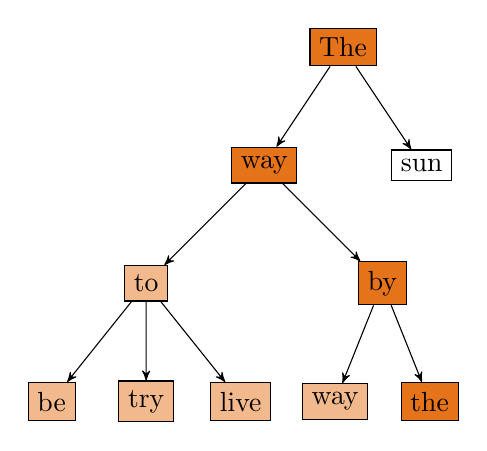
\begin{tikzpicture}[->,>=stealth',every node/.style={circle,draw},level 1/.style={sibling distance=20mm},level 2/.style={sibling distance=30mm},level 3/.style={sibling distance=12mm},
%scale=0.7, transform shape
]
\node [shape=rectangle,fill = orange!90!blue](nA){The}
   child { node[shape=rectangle,fill = orange!90!blue] (nB) {way}
              child { node[shape=rectangle,fill = orange!90!blue!50] (nD) {to}
                         child { node[shape=rectangle,fill = orange!90!blue!50] (nH) {be} }
                         	child { node[shape=rectangle,fill = orange!90!blue!50] (nI)  {try} }
                         child { node[shape=rectangle, fill = orange!90!blue!50] (nJ) {live} }
                       }
              child {  node [shape=rectangle,fill = orange!90!blue] (nE) {by}
                         child { node [shape=rectangle,fill = orange!90!blue!50] (nK) {way} }
                         child { node [shape=rectangle,fill = orange!90!blue] (nL) {the} }
                       }
            }
   child { node (nC) [shape=rectangle,] {sun}
           };

\end{tikzpicture}
}
\end{figure}

Our algorithm for resolution is an instantiation of depth first backtracking search. Because our rhyme constraints only are considered on the final word of a line, using depth first search is more efficient than using backtracking search for constraint checking and allows for rapid end-line state evaluation.

\begin{figure*} %change to figure if you don't want it to be full page
\caption{Search through corpus model with \emph{n} $= 2$}
\centering
\adjustbox{max width =\linewidth}{
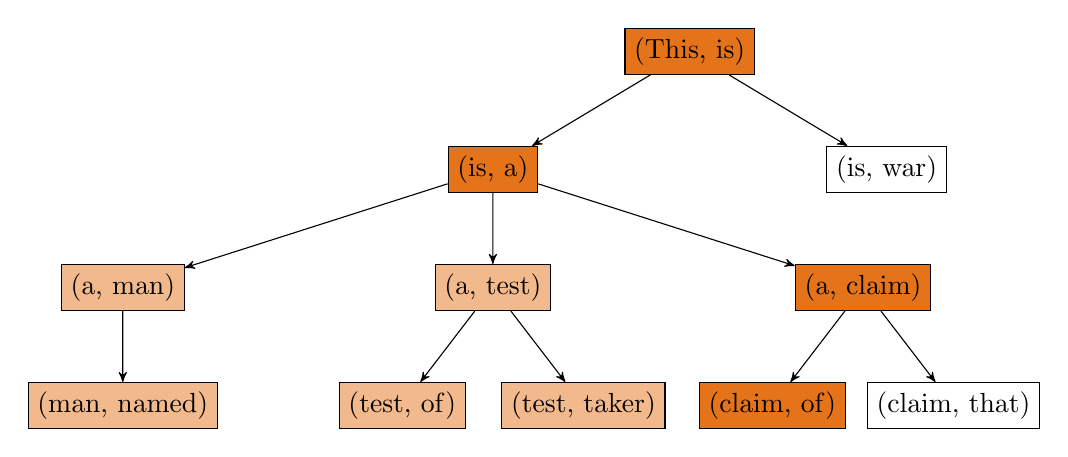
\begin{tikzpicture}[->,>=stealth',every node/.style={circle,draw},level 1/.style={sibling distance=50mm},level 2/.style={sibling distance=47mm},level 3/.style={sibling distance=23mm},
%scale=0.7, transform shape
]
\node [shape=rectangle,fill = orange!90!blue](nA){(This, is)}
   child { node[shape=rectangle,fill = orange!90!blue] (nB) {(is, a)}
              child { node[shape=rectangle,fill = orange!90!blue!50] (nD) {(a, man)}
                         child { node[shape=rectangle,fill = orange!90!blue!50] (nH) {(man, named)} }
                       }
              child { node[shape=rectangle,fill = orange!90!blue!50] (nM) {(a, test)}
                         child { node[shape=rectangle,fill = orange!90!blue!50] (nN) {(test, of)} }
                         child { node[shape=rectangle,fill = orange!90!blue!50] (nO) {(test, taker)} }
                       }
              child {  node [shape=rectangle,fill = orange!90!blue] (nE) {(a, claim)}
                         child { node [shape=rectangle,fill = orange!90!blue] (nK) {(claim, of)} }
                         child { node [shape=rectangle] (nL) {(claim, that)} }
                       }
            }
   child { node (nC) [shape=rectangle,] {(is, war)}
           };

\end{tikzpicture}
}
\end{figure*}

\section{Baseline}
Our baseline is a probabilistic \emph{n}-gram model that produces strings after being trained on an corpus. The baseline lacks rhyming constraints and semantic checking; however, it is able to produce rhetoric that uses the corpus' lexicon, relying on the \emph{n}-gram model to produce semantically consistent prose. As a simplifying assumption, the baseline assumes that a line of poetry has six words, as a stand-in for syllabic constraints. The first word of each line is based on the \emph{n}-gram value of the last n words on the previous line. Additionally, the baseline assumes that poetry has 15 lines and a standard form (same number of syllables per line, etc.). See appendix for output examples.

Our analysis of the output generated by the \emph{n}-gram model is that while the unigram model produces phrases that are grammatically and semantically inconsistent, the trigram model frequently just reproduces lines from the corpus verbatim. In the scope of the baseline, this may be a function of the size of the corpus alone, such that a trigram model may succeed at generating novel output once rhyming and syllabic constraints are imposed; however, it is also an indicator that unigram features alone may not be sufficient in order to produce novel grammatical output, depending on the size corpus. This prompted us to add additional syntactic feature indicators as we proceeded in our developmental process.

\section{Oracle}
The oracle for this problem is asking a human to write poetry, which we define as text satisfying constraints placed on syllable count and rhyme pattern. This is something that humans can do with high accuracy, creativity, and expression. For a given form (e.g. the sonnet), humans will be able to generate satisfactory output with almost 100\% accuracy if constraints on meaning or poetic quality are not in place. 

\section{Advanced Method}
Our advanced method performs depth-first-search over the \emph{n}-gram model in order to satisfy the constraints defined at runtime. We define this search problem as follows:
\begin{enumerate}
	\item \verb!startState!: (empty poem, \verb!-BEGIN-!), where \verb!-BEGIN-! is the initial seed of \emph{n}-gram language model
	\item \verb!action!: adding a valid word to the poem and updating the \emph{n}-gram seed
	\item \verb!isGoal(state)!: if poem is complete; all lines completed and constraints satisfied.
	\item \verb!succAndCost(state)!: returns a list of valid (word, (new poem, new seed), word frequency) tuples, where (new poem, new seed) is a successor pair for (poem, seed) that satisfies the constraints of the model (only valid actions taken). 
	\end{enumerate}
	
\subsection{Enforcing Constraints}
Principal among challenges we faced during development were formalizing the rhyme and syllabic constraints, specifically: how to incorporate these constraints into the model in order to direct the depth first search, how to evaluate the number of syllables in a word and how to determine if two words rhyme. Important for the success of our implementation was the utilization of Moby Python International Phonetic Alphabet (IPA) Dictionary \cite{Moby}. IPA readings of words represent their pronunciations in English, where each character represents a unique phoneme, or sound. 
\begin{enumerate}
\item \textbf{Algorithmic considerations}:The implementation of constraints is solved by a propagator-receiver framework in which end-line constraints are imposed in the forwards direction after a rhyme-propagating line is completed. For example, if lines 0 and 1 are designated to rhyme, then after the search has completed line 0, the rhyming constraint is propagated forwards onto line 1 (the receiver). This facilitates forward motion but also allows the algorithm to backtrack by arm's length when it is unable to resolve a constant by selecting a new rhyme to propagate forward after backtracking. 

\item \textbf{Syllable evaluation}: For each element of the IPA dictionary, the number of IPA vowels was counted and used as an estimate for the number of syllables in each word of the dictionary.  If a word in the corpus is not in the dictionary, an alternative estimate based upon word length is used. Most IPA transcriptions of words lacked digraphs (one vowel sound represented in IPA as multiple unicode symbols), resulting in a fairly accurate syllable estimate.

\item \textbf{Rhyme evaluation}: In our algorithm, the suffix for an entry in the IPA dictionary is defined as the substring starting at the consonant before last vowel in the word (if there is an antecedent consonant). Two words rhyme if their suffixes match. If one of the words is not in the IPA dictionary, a similar estimate is used based solely upon their standard alphabet spelling. Though rhyme detection is crucial to the success of the model, its development is auxiliary to the scope of our project as a whole. Thus, after experimenting with a number of syllable-estimation techniques, we found that this estimate was accurate for the majority of words output through generation.

\end{enumerate}
\subsection{Improving Content}
Additional algorithmic changes were made in order to make the output of the poem more semantically meaningful. In an attempt to increase the quality of poems generated, we took four approaches: grouping pairs of lines into semantic sentences, tracking beginning words in the \emph{n}-gram model in order to better approximate proper language, cleaning the corpora in order to remove extraneous words, and imposing part of speech constraints on the format of the poems.
\begin{table*}[t]
\caption{\textbf{Statistics run with -o 20 -t eight -l 2 -b 5 -r 5}}
\begin{adjustbox}{width=\linewidth}
\begin{tabular}{r | c | c c | c c | c | c}
Corpus & n & Mean Time (s) & Median Time (s) & Mean States & Median States & Completed & Score \\
\hline
\multirow{3}{*}{Eliot (1,268 lines)} & 1 & 91.66 & 66.84 & 4773.75 & 3547.5 & 100\% & 1.35 \\
& 2 & 0.21  & 0.18 & 163.05 & 111.5 & 0\% & \textemdash \\
& 3& 0.09 & 0.09 & 16.5 & 16 & 0\% & \textemdash \\ \hline
\multirow{3}{*}{Whitman (17,859 lines)} & 1 & 1352.69 & 165.729 & 4959.05 & 532 & 100\% & 1.66\\
&2 & 18.203 & 12.101 & 1705.6 & 1184 & 100\% & 2.45\\ 
& 3 & 1.548 & 1.415 & 80.2 & 60.5 & 0 & \textemdash \\ \hline
\multirow{3}{*}{Shakespeare (124,788 lines)} & 1 & 6480* & 6480* & 9333.80 & 397 & 100\% & 1.20*  \\
& 2 & 81.918 & 30.761 & 3784 & 1305.50 & 100\% & 2.18 \\ 
& 3 & 14.96 & 13.66 & 1220.90 & 1023 & 45\% & 3.22 \\ \hline

\multicolumn{8}{l}{\footnotesize *Only five poems generated after 9 hour run time; only these data points reported.}
\end{tabular}
\end{adjustbox}
\end{table*}

\begin{enumerate}
\item \textbf{Grouping lines into sentences}: Initially, our \emph{n}-gram model was trained on the entire corpus text unbroken. This led to the generator producing a continuous stream of text throughout the poem, which hindered semantic quality. To fix this, we added in the ability to reseed the poem anew after a given number of lines. Thus, the text in the poem was broken into smaller parts, allowing the poem to be composed of semantic sentences - streams of \emph{n}-gram generated text from separate seeds. This paved the way for other approaches to enforce meaning contained within distinct sentences. The frequency of reseeding is specifiable at runtime. 

\item \textbf{Changing seed behavior on new lines}: Even with the imposition of sentence structure on the poems, the meaning of the generated text was largely incomprehensible. A large reason for this was that the sentences would begin apparently in the middle of meaningful text, because the reseeding technique did not require the beginning of a sentence to represent the beginning of a phrase. To address this, special \verb!-BEGIN-! words were incorporated into the corpus between lines. This served two purposes: the \emph{n}-gram model would not remember following words for a seed if those words were part of a semantically separate sentence (we assumed that each line of the corpus was a separate sentence); and upon generation, the model could require that the starting seed for a new sentence be chosen from known sentence initiators.

\item \textbf{Corpus cleaning}: Certain corpora contain formatting or organizational phrases, e.g. verse and hook in song lyrics. Therefore, we added the possibility to tailor the \emph{n}-gram model to different corpus sources by trimming these extraneous phrases from the corpus before analyzing it.

\item \textbf{Part-of-speech constraints}: Well-formed English sentences generally do not end with conjunctions, articles, or prepositions. Using open-source English dictionaries mapping words to their possible parts of speech in sentences, we determined whether the words in our reference dictionary were used as conjunctions, articles, or prepositions.\cite{Moby} When evaluating a potential end-of-line word, if the word was one of these parts of speech,  we did not add it to the line.
\end{enumerate}

\subsection{Improving Runtime}
Finally, when testing our program, we began to notice that the program would sometimes go down a path that could not satisfy the constraints. For nodes in the \emph{n}-gram model with a large number of children, the algorithm would loop through every single one in order to see if it satisfied the constraints before backtracking. We implemented a branching constraint that restricts the amount of children that the depth-first search explores before backtracking. This prunes the search space and enables the algorithm to backtrack to the previous line to select a new rhyming word without testing the entire sub-tree. With a low branching limit, the search fails earlier and backtracks more quickly, though this behavior may not always be desirable. 

\begin{figure*}[th]
\caption{Median runtime, median explored states, meaningfulness scores vs. n-gram model order}
\centering
\begin{adjustbox}{width=\linewidth}
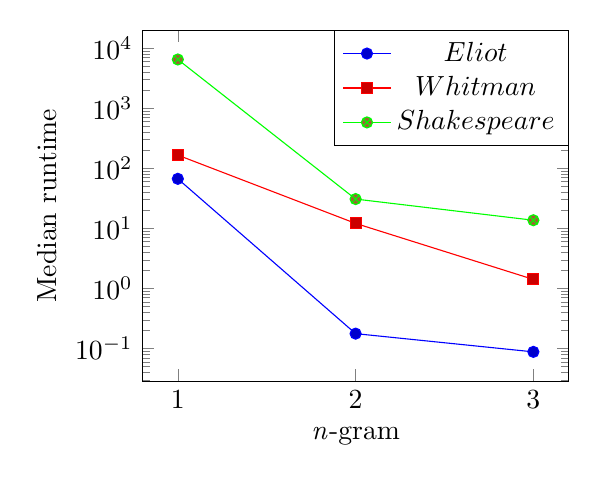
\begin{tikzpicture}
    \begin{axis}
        [
        ,width=7cm
        ,xlabel=\emph{n}-gram
        ,ylabel=Median runtime
        ,ymode=log
        ,xtick=data,
        ,legend style={at={(1,1)},
  				anchor=north east}
       %,xtick={0,1,...,3}
        ,%xticklabels={Test A,Test B,Test C,Test D}
        ]
        \addplot+[sharp plot, color = blue] coordinates
        {(1,66.844) (2,0.177) (3,0.088)};
        \addplot+[sharp plot, color = red] coordinates
        {(1,165.729) (2,12.101) (3, 1.415)};
         \addplot+[sharp plot, color = green] coordinates
        {(1, 6480) (2,30.761) (3,13.661)};
        \legend{$Eliot$,$Whitman$,$Shakespeare$}
      \end{axis}
\end{tikzpicture}
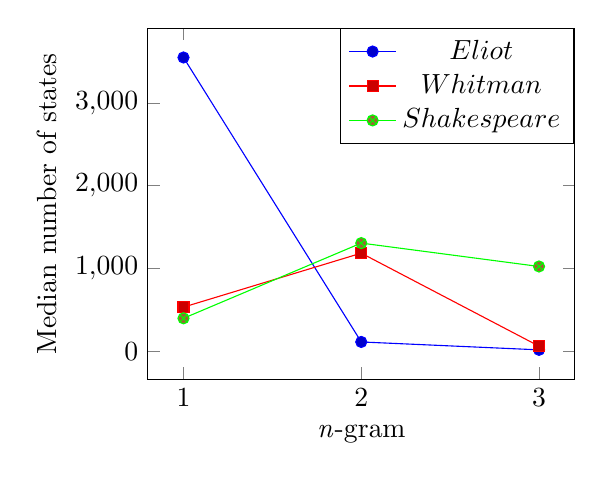
\begin{tikzpicture}
    \begin{axis}
        [
        ,width=7cm
        ,xlabel=\emph{n}-gram
        ,ylabel=Median number of states
        ,xtick=data,
        ,legend style={at={(1,1)},
  				anchor=north east}
       %,xtick={0,1,...,3}
        ,%xticklabels={Test A,Test B,Test C,Test D}
        ]
        \addplot+[sharp plot, color = blue] coordinates
        {(1,3547.5) (2,111.5) (3,16)};
        \addplot+[sharp plot, color = red] coordinates
        {(1,532) (2,1184) (3, 60.5)};
         \addplot+[sharp plot, color = green] coordinates
        {(1,397) (2,1305.5) (3,1023)};
        \legend{$Eliot$,$Whitman$,$Shakespeare$}
      \end{axis}
\end{tikzpicture}
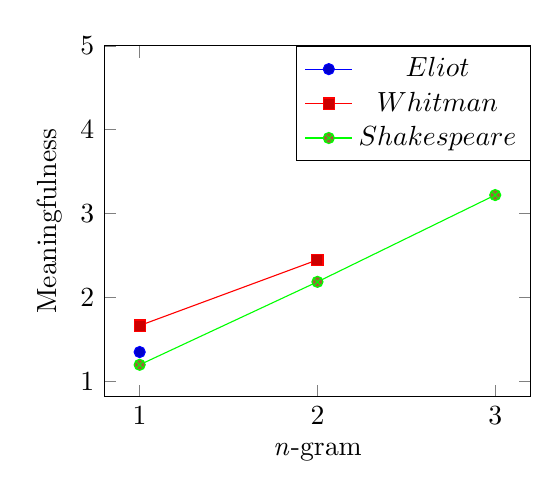
\begin{tikzpicture}
    \begin{axis}
        [
        ,width=7cm
        ,xlabel=\emph{n}-gram
        ,ylabel=Meaningfulness
        ,legend style={at={(1,1)},
  				anchor=north east}
       ,xtick={1,...,3}
       ,ymax=5
        ,%xticklabels={Test A,Test B,Test C,Test D}
        ]
        \addplot+[sharp plot, color = blue] coordinates
        {(1,1.352)};
        \addplot+[sharp plot, color = red] coordinates
        {(1,1.667) (2,2.45)};
         \addplot+[sharp plot, color = green] coordinates
        {(1,1.2) (2,2.188) (3,3.222)};
        \legend{$Eliot$,$Whitman$,$Shakespeare$}
      \end{axis}
\end{tikzpicture}

\end{adjustbox}
\end{figure*}

\section{Data \& Experiments}
To analyze our algorithm, we varied our algorithmic parameters (order of the Markov model) and input sources (training corpus) and observed the impact on: time required to completion, space required for completion, completion rate, and semantic scoring. 

Time, measured in seconds, was calculated by the computer running our algorithm, a Barley computer through Stanford FarmShare. The space required for completion was calculated as the number of states explored; in other words, the number of candidate words tested before completing the solution poem. The semantic scoring for poems was calculated by asking human reviewers to rate the poems on a scale from 1 to 5, where 1 denoted gibberish and a 5 denoted an excellent poem. 

For each trial, the algorithm attempted to satisfy twenty poems, with a specified Poetry model consisting of eight lines with ten syllables per line and the rhyming constraints \verb+AABBCCDD+. Above is a summary of the effects of our two independent variables. Our reseed limit was set to 5, meaning that our algorithm tried up to five \verb!-BEGIN-! words to start each sentence before returning that no solution could be found. Our branching limit was also set to 5, meaning that only five candidate words would be tried for any particular n-gram node before backtracking.

\subsection{Varying N-gram}
In our analysis we used unigram, bigram, and trigram functions (we found that almost no corpora would produce output when quadgram or higher was used). As the value of n increased, the time required for completion decreased, the space required for completion decreased, the percentage of successful solutions found decreased, and the average semantic score of the output increased. This matches our predictions, as increasing the value of n decreases the number of viable next-word candidates. Thus, there is a smaller state space, which means that solutions (if they exist) will be found more rapidly. However, this leaves fewer possible solutions, so the completion percentage of poems decreases: we find that only one corpus was able to generate any poems at $n=3$. As n increases, the text becomes more representative of human-generated English, so as expected the poems become more sensical and coherent.

\begin{table*}[th]
\caption{\textbf{Varying branching limit with n=3}}
\label{table:a}
\begin{adjustbox}{width=\linewidth}
\begin{tabular}{r | c | c c | c c | c | c}
Corpus & Branching & Mean Time (s) & Median Time (s) & Mean States & Median States & Completed & Score \\ \hline
\multirow{2}{*}{Whitman (17,859 lines)} & 5 & 1.548 & 1.415 & 80.2 & 60.5 & 0\% & \textemdash\\
&\textemdash & 3.48 & 2.22 & 1759.85 & 172 & 15\% & 3.67\\ \hline
\multirow{2}{*}{Shakespeare (124,788 lines)} & 5 & 14.96 & 13.66 & 1220.90 & 1023 & 45\% & 3.22 \\
& \textemdash & 21.85 & 20.727 & 5699.45 & 4159 & 85\% & 3.38 \\ \hline
\end{tabular}
\end{adjustbox}
\end{table*}

\subsection{Varying Input Sources}
The input sources used varied in size roughly by a factor of 10: small (T.S. Eliot, $10^3$ lines), medium (Walt Whitman, $10^4$ lines), and large (Shakespeare, $10^5$ lines). All of the sources were poetry. Increasing the corpus size increased the time required to completion, states required for completion, completion percentage, but did not affect the semantic score. With a larger corpus, the search state space increases, so the time and space required to find a solution also increase. As there are more possible solutions, the completion percentage also increases. The semantic rating did not appear to be affected by the size of the corpus; we would expect the content as well as than quantity of the text to impact this variable. 

%\begin{figure}[t]
%\caption{Median explored states vs. n-gram model order}
%\centering
%\begin{tikzpicture}
%    \begin{axis}
%        [
%        ,width=7cm
%        ,xlabel=\emph{n}-gram
%        ,ylabel=Median number of states
%        ,xtick=data,
%        ,legend style={at={(1,1)},
%  				anchor=north east}
%       %,xtick={0,1,...,3}
%        ,%xticklabels={Test A,Test B,Test C,Test D}
%        ]
%        \addplot+[sharp plot] coordinates
%        {(1,532) (2,1184) (3, 60.5)};
%         \addplot+[sharp plot] coordinates
%        {(1,397) (2,1305.5) (3,1023)};
%        \addplot+[sharp plot] coordinates
%        {(1,3547.5) (2,111.5) (3,16)};
%        \legend{$Whitman$,$Shakespeare$,$Eliot$}
%      \end{axis}
%\end{tikzpicture}
%\end{figure}
%
%\begin{figure}
%\caption{Meaningfulness score vs. n-gram model order}
%\centering
%\begin{tikzpicture}
%    \begin{axis}
%        [
%        ,width=7cm
%        ,xlabel=\emph{n}-gram
%        ,ylabel=Meaningfulness
%        ,legend style={at={(1,1)},
%  				anchor=north east}
%       ,xtick={1,...,3}
%       ,ymax=5
%        ,%xticklabels={Test A,Test B,Test C,Test D}
%        ]
%        \addplot+[sharp plot] coordinates
%        {(1,1.667) (2,2.45)};
%         \addplot+[sharp plot] coordinates
%        {(1,1.2) (2,2.188) (3,3.222)};
%        \addplot+[sharp plot] coordinates
%        {(1,1.352)};
%        \legend{$Whitman$,$Shakespeare$,$Eliot$}
%      \end{axis}
%\end{tikzpicture}
%\end{figure}


\subsection{Branching Limit Analysis}
Additionally, tests were run in order to examine the effects that the branching limit had on performance. Intuitively, we expected that removing the branching limit would increase the number of solutions found, but were interested to see the effect of removing the limit at the expense of time and space. We ran the algorithm on Whitman and Shakespeare with $n=3$ with no branching limit in place and compared the results to the results we conducted earlier. We found that for the smaller corpus, Whitman, the effect was rather small, with only 3 additional poems terminating. For the larger corpus, the effect was much more visible, with the algorithm finding a solution 85\% of the time. To us, this indicates that the branching limit should scale with both the size of the corpus and the order of the \emph{n}-gram model. As the size of the corpus increases, there are more possible nodes of the \emph{n}-gram model that may yield a solution. Similarly, as the order of the \emph{n}-gram model increases, the fewer children each node has, so discarding some of the children paths becomes more costly. Removing the branching factor increased runtime and space analysis by approximately the same factor for both corpora, see table \ref{table:a} above.

\subsection{Progress Analysis}

Table \ref{table:b} below shows the progress we have made after implementing our search algorithm, showing statistics for the same corpus run with n = 3 using each technique. While the algorithm has nearly mastered the process of making rhyming pairs and meeting syllable restrictions, smaller gains were made on the meaningfulness metric. This demonstrates what a difficult problem semantic generation is for researchers, but also demonstrates the level of forward progress that can be made by implementing further constraints on the algorithm. 

\begin{table}[h]
\caption{\textbf{Two approaches to Whitman}}
\label{table:b}
\begin{adjustbox}{width=\linewidth}
\begin{tabular}{c | c | c | c}
Algorithm & Meaningfulness & \% Correct Rhyme & \% Correct Syllable \\ \hline
Baseline & 1.55 & 2.50\% & 12.50\% \\
Advanced & 3.67 & 96.25\% & 98.75\% \\ \hline
\end{tabular}
\end{adjustbox}
\end{table}

\section{Conclusion \& Further Work}
Our project generated poetry with surprising quality that managed to convince some readers that it was written by humans, achieving our initial goal. However, there are several directions for further work. 
\begin{enumerate}
\item \textbf{Syllabic stress}: Some forms of human poetry place requirements on syllabic stress patterns: one example is iambic pentameter, requiring that stressed and unstressed syllables be altered. Given the phonetic rendering for a written word, one can determine the stressed and unstressed syllables and thus meet constraints on syllabic stress patterns in addition to syllabic count. One difficulty with meeting syllabic constraints on text is that a given word can be pronounced in multiple ways, some of which are preferable in particular contexts. Nevertheless, the area still holds potential for exploration and allows for poems to meet even more fine-grained constraints. 
\item \textbf{Pseudo-grammatical structure}: One heuristic we used to improve our poem was placing a part of speech constraint on the final word of a line, based on what occurs in English. We could extend this practice by placing other part of speech constraints on lines or sentences. For example, we could stipulate that verbs not begin sentences, each line have a certain number of lines, have sentences that follow established generative syntactic patterns, etc.
\item \textbf{Topical generation}: Some projects in the field attempted to generate poems about a particular topic, rather than in the style of a particular poet. We could allow the user to specify a topic word, and enforce that the poem meet some constraints making it related to the topic. A naive constraint is that the word actually appear in the poem; further investigation may reveal more complex relationships.
\item \textbf{Runtime efficiency}: One possibility for shortening the runtime of the algorithm is to use reverse-looking Markov chains to begin lines with the final (rhyming) words, then fill in the subsequent words. This would require more preprocessing of the corpus data to properly generate chains, which may not actually enhance the total time to generate a poem when given an arbitrary corpus; further investigation is necessary. 
\item \textbf{Extending rhyme vocabulary}: Unfortunately, the model does not always produce results, and this is primarily a result of corpora that are small enough that the \emph{n}-gram generator cannot find rhyming pairs. In order to solve this problem, we had ideas of re-analyzing the corpus, calculating rhyming words for all of the words in the corpus, and supplementing the corpus with additional words in order to facilitate rhyme-finding. This would allow the constraints to be satisfied in a more efficient manner by relaxing the way that words are selected (reducing the rigidity of the lexicon) in order to choose rhyming nouns outside of the corpus. This could potentially decrease the influence of the corpus, especially if too liberal a policy is implemented, but balancing the preservation of the corpus against relaxation remains an area that is worthy of exploration.
\end{enumerate}

\begin{thebibliography}{10}

\bibitem{bot} Bot or not. \\
 \begin{adjustbox}{width=\linewidth}\verb+http://botpoet.com/what-is-computer-poetry/+\end{adjustbox}

\bibitem{seuss} Capnrefsmmat/seuss. \begin{adjustbox}{max width=\linewidth}\verb+https://github.com/capnrefsmmat/seuss+\end{adjustbox}

\bibitem{Dunning} Dunning, T. (1994). Statistical identification of language (pp. 10-03). Computing Research Laboratory, New Mexico State University.

\bibitem{Kurzweil} Kurzweil, R. A (Kind of) Turing Test. \begin{adjustbox}{width=\linewidth}\verb+http://www.kurzweilcyberart.com/poetry/rkcp_akindofturingtest.php+\end{adjustbox}

\bibitem{Gutenberg} Project Gutenberg.\verb+http://www.gutenberg.org/+

\bibitem{Moby} The Institute for Language, Speech and Hearing. \verb+http://icon.shef.ac.uk/Moby/+

\bibitem{Toivanen} Toivanen, J., Toivonen, H., Valitutti, A., \& Gross, O. (2012). Corpus-based generation of content and form in poetry. In Proceedings of the Third International Conference on Computational Creativity.

\end{thebibliography} 
\pagebreak
\clearpage
\begin{appendices}
\section{Example Poems}
\subsection{Baseline}
\subsubsection{Eliot}
\begin{alltt}
She turned away, but with the
palms turned out, Chicago Semite Viennese.
A lustreless protrusive eye Stares from
the damp savannas, And quiring angels
round him sing The praise of
God, in loud hosannas. Blood of
the street, Rubbing its back upon
the floor She yawns and draws
\end{alltt}

\subsubsection{Shakespeare}

\begin{alltt}
thee. I prithee give me a
paper LONGAVILLE. By whom this vile
deed We must to the source
from whence thou com'st. Suppose the
singing birds musicians, The grass whereon
thou tread'st the presence of the
great seal presently Into our presence,
where their lord should be so
\end{alltt}

\subsection{n=1}
\subsubsection{Eliot}
\begin{alltt}
under a man with such was there
was such knowledge what have the hair
she has left him shall i am not
reached conclusion when do i bought
and leave it toward the lady
in its tongue into the body
before the bed is to light crept
up high and indeed i have wept
\end{alltt}

\begin{alltt}
a question on his hair of high
and he shall i had such a dry
with such hair too--so the water
all what she came through the waiter
are the brown waves of smoky days
and of sweeney shifts from the praise
in the prince no great aunts were not
knowing what she smiles and the lot
\end{alltt}

\subsubsection{Whitman}
\begin{alltt}
something startles me the poems
churches i was strewn in freedoms
the present all teachers and far
advanced and what the core of are
with his gray and the power wealth
clothes from the sight in him by stealth
to sing on the greater or i
am he swims through the long at high
\end{alltt}

\subsubsection{Shakespeare}
\begin{alltt}
i choose wrong lord i have stayd us
now is a sigh away she thus
a beard they fight for your sake send
it only painted clay and end
first murtherer a mind i dare
not yet methinks you dwell with fair
a forerunner my tent and gave
him better here must be so brave
\end{alltt}

\subsection{n=2}

\subsubsection{Whitman}
\begin{alltt}
hear the sounds there also sounding
the howl of the earth expanding
and i or you are sick as they
who give the hearts of the globe lay
as down the storm shall dash thy face
the limbs of the sea in the race
the simple house of himself or
herself not for life and the war
\end{alltt}

\begin{alltt}
will make the songs of the glory
of the race and of the merry
from the hour of death the great
spheres time and space i him dilate
i see the harpooneer standing
up i see the shells exploding
the love of the most friends for i
know very well i could not die
\end{alltt}

\subsubsection{Shakespeare}
\begin{alltt}
the king is dead we will not stay	
behind you my lord i should say
and he to yours and all of you
to you and you and you sir hugh
when they are gone then must i think
you know my lord i dare not drink
king ay that there is this jewel
in the world i had my trial
\end{alltt}

\subsection{n=3}
\subsubsection{Whitman}
\begin{alltt}
what do you think a great city
is that which has the quality
i sing the songs of the glory
of the race and of the merry
now i see what you do not say
they are not vile any more they
the love of the most friends for i
know very well i could not die
\end{alltt}

\subsubsection{Shakespeare}
\begin{alltt}
king henry for my part i care
not i knew she and all the fair
and speak i will i will and ill
be revengd on him for he will
and use it for my part i care
not i knew she and all the fair
up in my heart to her but i
love thee and when i have been dry
\end{alltt}

\begin{alltt}
in despite of all that i can
tell you that which you are a man
i will be so bold as to tell
you that i am not mad too well
doug as heart can think there is not
a thing to you there is a plot
this be not that she will not come
to thee for i have seen the dumb
\end{alltt}
\newpage
\section{More examples}
\subsection{Kanye West, n=2}
\begin{alltt}
my check say lost my soul to keep
the strong around me they say sleep
but my link had me on the real
people i could do it i feel
you dont want to do this at home
with me baby you a new rome
i can tell you where i came back
for you that say yes he was black
\end{alltt}

\subsection{Plato, sonnet, n=2}
\begin{alltt}
must follow up what he is the very
light of heaven he said i think is quite
and what are these two as in a fury
of passions and desires this is right
the interest of the process and look sharp
that justice is any one in the state
the city which he is good and the harp
the harp-player as in the state all great
sense must acknowledge that bad and good will
be the education of our rules
the god should ever be known to be still
worse if you are quite right he said the tools
he will having first chained up the state falls
sick and the maker of the one who calls
\end{alltt}

\subsection{Collection of Frank Ocean haikus, n=2}
\begin{alltt}
gimme it now hear
me out just hear me out just
no dont ever leave

and a new day will
bring another crying babe
im wherever you

this life goes on man
thats one thing about this world
and when im standing
\end{alltt}
\end{appendices}


\end{document}